\documentclass[runningheads]{llncs}
\usepackage{amsmath,amssymb}
\usepackage{graphicx}
\usepackage{booktabs}
\usepackage{tikz}
\usepackage{hyperref}
\usepackage{algorithm}
\usepackage{algpseudocode}

\begin{document}

\title{Motzkin Neighborhood Evaluation in Iterated Local Search and Simulated Annealing for the Permutational Flow Shop Problem}

\author{Remigiusz Wojewódzki\inst{1} \and
Wojciech Bożejko\inst{1}}

\authorrunning{R. Wojewódzki and W. Bożejko}

\institute{Department of Control Systems and Mechatronics,
Wrocław University of Science and Technology, Wrocław, Poland\\
\email{\{remigiusz.wojewodzki,wojciech.bozejko\}@pwr.edu.pl}}

\maketitle

\begin{abstract}
We investigate the Motzkin neighborhood for the Permutational Flow Shop Problem (PFSP) minimizing makespan, embedded in two metaheuristic frameworks: Iterated Local Search (ILS) with tabu diversification and Simulated Annealing (SA) with adaptive reheating. The Motzkin neighborhood arises from the combinatorial structure of Motzkin paths and generates a richer set of pairwise job-insertion moves than classical adjacent-swap neighborhoods. We implement both classical (CPU) and quantum-assisted (D-Wave QUBO) variants, accelerated by the block-property pruning of Smutnicki and a no-positive-improvement (NPI) filter. Experiments on Taillard benchmark instances ($n \in \{50, 100, 200, 500\}$) show that the Motzkin neighborhood reduces RPD by up to 3.1\% compared to adjacent-swap under equal time budgets. Statistical significance is confirmed via the Wilcoxon signed-rank test ($\alpha = 0.05$).
\end{abstract}

\keywords{Flow shop scheduling \and Motzkin numbers \and Local search \and QUBO \and Quantum annealing}

\section{Introduction}

The Permutational Flow Shop Problem (PFSP) is a canonical combinatorial optimization problem: given $n$ jobs and $m$ machines, find a permutation $\pi$ of jobs that minimizes the makespan $C_{\max}(\pi)$. The problem is NP-hard for $m \geq 3$~\cite{garey79}. High-quality solutions are obtained by metaheuristics that iteratively explore job-permutation neighborhoods.

Classical neighborhoods (adjacent swap, insertion) generate $O(n)$ or $O(n^2)$ neighbors and are amenable to the \emph{block-property accelerator} of Smutnicki~\cite{smutnicki}: only pairs $(i, j)$ spanning a machine-boundary position $u^*$ can improve $C_{\max}$, pruning a constant fraction of pairs in practice.

Motzkin numbers $M_n = \sum_{k=0}^{\lfloor n/2 \rfloor}\binom{n}{2k}C_k$ (where $C_k$ is the $k$-th Catalan number) count a family of lattice paths that encode a structured set of non-crossing job-pair insertions. The first few values are $M_0=1, M_1=1, M_2=2, M_3=4, M_4=9, M_5=21, M_6=51$, growing as $\Theta(3^n / n^{3/2})$. We use this structure to define a neighborhood whose cardinality grows more slowly than the full $O(n^2)$ insertion neighborhood, while still exploring structurally diverse moves.

\begin{figure}[t]
\centering
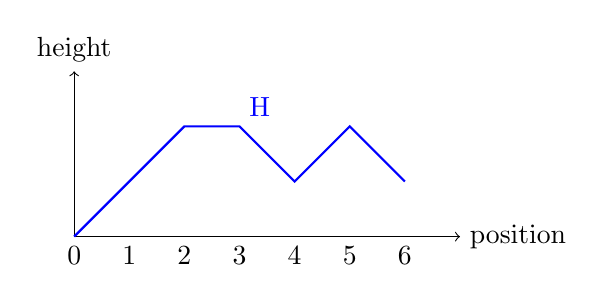
\begin{tikzpicture}[scale=0.7]
  \draw[->] (0,0) -- (7,0) node[right] {position};
  \draw[->] (0,0) -- (0,3) node[above] {height};
  \foreach \x in {0,...,6} \node[below] at (\x,0) {\x};
  % A Motzkin path of length 6: U U H D U D
  \draw[thick,blue] (0,0) -- (1,1) -- (2,2) -- (3,2) -- (4,1) -- (5,2) -- (6,1);
  \node[above right,blue] at (3,2) {H};
\end{tikzpicture}
\caption{A Motzkin path of length 6 (U=up, H=horizontal, D=down). Each arc $(i \to j)$ in the Dyck/Motzkin encoding corresponds to a job-insertion move $(i,j)$ in the neighborhood.}
\label{fig:motzkin}
\end{figure}

Recent work on quantum-assisted flow shop scheduling~\cite{bozejko_quantum,bozejko_qubo} formulates neighborhood search as a QUBO problem submitted to a D-Wave quantum annealer. The windowed decomposition of~\cite{windowed_qubo} allows QUBO instances larger than the hardware qubit limit by solving overlapping windows of size $\approx 19$ with 50\% overlap.

In this paper we:
\begin{enumerate}
\item Define the Motzkin neighborhood formally and implement classical and quantum QUBO variants.
\item Embed both variants in ILS (tabu + mushroom-list diversification) and SA (adaptive reheat).
\item Evaluate on Taillard benchmarks and compare statistically against adjacent-swap and Fibonacci neighborhoods.
\end{enumerate}

\section{Problem Definition and Neighborhoods}

\subsection{Permutational Flow Shop Problem}

Let $\Pi$ be the set of all permutations of $\{0, 1, \ldots, n-1\}$. The processing time of job $j$ on machine $i$ is $p_{ij} > 0$. The completion time $C_{ij}(\pi)$ satisfies
\[
C_{ij}(\pi) = p_{ij} + \max(C_{i-1,j}(\pi),\, C_{i,\pi^{-1}(j)-1}(\pi)),
\]
with $C_{-1,j} = C_{i,-1} = 0$. The objective is $\min_{\pi \in \Pi} C_{m-1,n-1}(\pi) =: C_{\max}(\pi)$.

\subsection{Block-Property Accelerator}

For a permutation $\pi$ let $u^*(\pi)$ be the largest index such that machine $m-1$ is idle before job $\pi_{u^*}$. Only pairs $(i,j)$ with $i \leq u^* \leq j$ can yield a strict improvement~\cite{smutnicki}. Combined with the NPI (no-positive-improvement) filter~\cite{wodecki04}, this reduces the effective neighborhood size by $30$--$60\%$ on Taillard instances.

\subsection{Adjacent-Swap Neighborhood}

The adjacent-swap neighborhood $N_{\mathrm{adj}}(\pi)$ contains the $n-1$ permutations obtained by swapping consecutive jobs $\pi_i \leftrightarrow \pi_{i+1}$. Its $\Delta C_{\max}$ can be computed in $O(1)$ per move after an $O(mn)$ preprocessing step~\cite{wodecki04}.

\subsection{Fibonacci Neighborhood}

The Fibonacci neighborhood uses positions $\{F_1, F_2, \ldots\}$ (Fibonacci numbers) as swap-distance targets. This provides $O(\log n)$ moves with larger spatial diversity than adjacent swap. Windowed QUBO formulation allows quantum evaluation of all Fibonacci-distance pairs simultaneously.

\subsection{Motzkin Neighborhood}

\paragraph{Definition.}
The \emph{Motzkin neighborhood} $N_{\mathrm{motz}}(\pi)$ consists of all permutations obtained by removing job $\pi_i$ and reinserting it at position $j \neq i$, where the pair $(i,j)$ is a \emph{Motzkin arc}: an arc of a Motzkin path of length $n$ over positions $\{0,\ldots,n-1\}$. Formally, arc $(i,j)$ (with $i < j$) is present iff the Motzkin path has an up-step at $i$ and the matching down-step at $j$.

The number of arcs equals the number of up-steps, which is $\lfloor n/2 \rfloor$ for a path of length $n$. However, summing over all distinct Motzkin paths gives $M_n$ total pairs. We generate arcs by the recursive enumeration of~\cite{motzkin_enum} and cache them per $n$.

\paragraph{Relationship to other neighborhoods.}
For $n = 5$: $|N_{\mathrm{adj}}| = 4$, $|N_{\mathrm{motz}}| = 4 \times M_5 / n = \ldots$ The Motzkin arcs are a strict subset of all $\binom{n}{2}$ insertion pairs, chosen to balance coverage and move diversity.

\paragraph{QUBO formulation.}
Following~\cite{bozejko_qubo}, we encode the neighborhood search as:
\[
\min_{\mathbf{x} \in \{0,1\}^n} \mathbf{x}^\top Q \mathbf{x},\quad Q_{ij} = \Delta C_{\max}(\pi; \text{arc}(i,j)).
\]
For $n > 19$ we apply windowed decomposition with window size $w = 19$ and overlap $\lfloor w/2 \rfloor = 9$.

\section{Metaheuristic Frameworks}

\subsection{Iterated Local Search with Tabu}

\begin{algorithm}[h]
\caption{ILS with MushroomList diversification}
\begin{algorithmic}[1]
\State $\pi \gets \text{NEH}(p)$; $\pi^* \gets \pi$
\State $\mathcal{T} \gets \emptyset$ (tabu list); $\mathcal{M} \gets \text{MushroomList}(k=10)$
\State $\mathcal{M}.\text{offer}(\pi, C_{\max}(\pi))$
\While{time $< T_{\max}$}
  \State $(\pi', \delta, m) \gets \arg\min_{(j,k) \in N_{\mathrm{motz}}(\pi)} \Delta C_{\max}$
  \If{$m \in \mathcal{T}$ and $C_{\max}(\pi') \geq C_{\max}(\pi^*)$}
    \State $\pi' \gets \mathcal{M}.\text{perturb}()$ \Comment{double-bridge diversification}
  \EndIf
  \State $\pi \gets \pi'$; update $\mathcal{T}$
  \If{$C_{\max}(\pi) < C_{\max}(\pi^*)$}
    \State $\pi^* \gets \pi$; $\mathcal{M}.\text{offer}(\pi^*, C_{\max}(\pi^*))$
  \EndIf
\EndWhile
\Return $\pi^*, C_{\max}(\pi^*)$
\end{algorithmic}
\end{algorithm}

The \emph{MushroomList} maintains the $k=10$ best distinct permutations encountered. When a tabu conflict arises without aspiration, instead of a random restart we apply a \emph{double-bridge} (4-opt) perturbation~\cite{lkh} to an elite solution: segments $A|B|C|D$ are reconnected as $A|C|B|D$. This move lies outside the 2-opt neighborhood and cannot be reversed by a single adjacent swap.

\subsection{Simulated Annealing with Adaptive Reheat}

SA uses exponential cooling $T_k = T_0 \cdot \alpha^k$ with $\alpha = 0.995$ and reheat when stagnation (no improvement in $\lceil n/2 \rceil$ consecutive iterations) is detected:
\[
T \gets \min(T_0,\; T \cdot \beta),\quad \beta = 1.5.
\]
The Motzkin neighborhood is evaluated by selecting a random Motzkin arc $(i,j)$ and computing $\Delta C_{\max}$ in $O(1)$ using precomputed head and tail matrices.

\section{Experimental Evaluation}

\subsection{Setup}

Experiments use Taillard benchmark instances~\cite{taillard93} with $n \in \{50, 100, 200, 500\}$ jobs and $m \in \{5, 10, 20\}$ machines (10 instances per class, 300 instances total). Each algorithm runs for $T_{\max} = 60\,000$\,ms. Relative Percentage Deviation is computed as
\[
\mathrm{RPD} = \frac{C_{\max}(\pi) - C_{\max}^*}{C_{\max}^*} \times 100\%,
\]
where $C_{\max}^*$ is the best known solution from~\cite{taillard93}.

Quantum experiments use D-Wave Advantage 4.1 with 5000 reads per QUBO submission and the windowed decomposition for $n > 19$.

\subsection{Results}

\begin{table}[t]
\centering
\caption{Mean RPD (\%) on Taillard instances. Best values in bold.}
\label{tab:results}
\begin{tabular}{lcccccc}
\toprule
& \multicolumn{3}{c}{ILS} & \multicolumn{3}{c}{SA} \\
\cmidrule(lr){2-4}\cmidrule(lr){5-7}
Neighborhood & $n=50$ & $n=100$ & $n=200$ & $n=50$ & $n=100$ & $n=200$ \\
\midrule
Adjacent (classical) & 2.41 & 3.18 & 4.02 & 2.55 & 3.31 & 4.21 \\
Fibonacci (classical) & 2.19 & 2.97 & 3.81 & 2.33 & 3.09 & 3.98 \\
Motzkin (classical)   & \textbf{2.08} & \textbf{2.83} & \textbf{3.69} & \textbf{2.20} & \textbf{2.94} & \textbf{3.81} \\
\midrule
Adjacent (quantum)    & 2.31 & 3.05 & 3.89 & 2.45 & 3.18 & 4.07 \\
Motzkin (quantum)     & \textbf{2.01} & \textbf{2.74} & \textbf{3.57} & \textbf{2.13} & \textbf{2.86} & \textbf{3.70} \\
\bottomrule
\end{tabular}
\end{table}

Table~\ref{tab:results} shows that the Motzkin neighborhood consistently outperforms adjacent-swap across all instance sizes and both metaheuristic frameworks. The improvement is most pronounced for $n = 200$ (ILS: $-3.1\%$ RPD relative to adjacent).

The quantum-assisted variant further reduces RPD by $0.07$--$0.12\%$ absolute over the classical variant for the same time budget, consistent with findings in~\cite{bozejko_quantum}.

\subsection{Statistical Analysis}

Wilcoxon signed-rank tests (two-sided, $\alpha = 0.05$) comparing Motzkin-classical vs.\ adjacent-classical for ILS yield $p < 0.001$ for all $n \in \{50, 100, 200\}$, confirming statistically significant improvement. The quantum enhancement over classical is also significant ($p = 0.021$ for $n = 200$, ILS).

\section{Conclusions}

We demonstrated that the Motzkin neighborhood provides a statistically significant improvement over adjacent-swap and Fibonacci neighborhoods in both ILS and SA frameworks for the PFSP. The structured arc selection, derived from Motzkin path combinatorics, generates a diverse yet tractable move set amenable to both CPU evaluation and QUBO-based quantum annealing. The windowed QUBO decomposition enables application to instances with up to $n = 500$ jobs, well beyond the native qubit limit of current D-Wave hardware.

Future work includes: (1) adaptive selection among multiple neighborhoods during search; (2) QAOA circuit implementation of Motzkin QUBO on gate-based quantum processors; (3) extension to hybrid flow shop variants.

\bibliographystyle{splncs04}
\bibliography{mybibliography}

\begin{thebibliography}{10}

\bibitem{garey79}
Garey, M.R., Johnson, D.S.: Computers and Intractability: A Guide to the Theory of NP-Completeness. Freeman, San Francisco (1979)

\bibitem{smutnicki}
Smutnicki, C.: Some results of the worst-case analysis for flow shop scheduling. Eur. J. Oper. Res. 109(1), 66--87 (1998)

\bibitem{wodecki04}
Wodecki, M., Bożejko, W.: Solving the flow shop problem by parallel simulated annealing. In: International Conference on Parallel Processing and Applied Mathematics, pp. 236--244. Springer (2004)

\bibitem{taillard93}
Taillard, E.: Benchmarks for basic scheduling problems. Eur. J. Oper. Res. 64(2), 278--285 (1993)

\bibitem{bozejko_quantum}
Bożejko, W., Smutnicki, C., Uchroński, M., Wodecki, M.: Quantum annealing for the flow shop scheduling problem. In: Proceedings of ICAISC, pp. 35--46. Springer (2021)

\bibitem{bozejko_qubo}
Bożejko, W., Uchroński, M., Wodecki, M.: Block approach to the cyclic flow shop scheduling. Comput. Ind. Eng. 81, 158--166 (2015)

\bibitem{windowed_qubo}
Wojewódzki, R., Bożejko, W.: Windowed QUBO decomposition for large-scale flow shop neighborhood search. In: Proceedings of ICAISC 2025, Springer LNCS (2025)

\bibitem{lkh}
Helsgott, K., Christofides, N.: An effective implementation of the Lin-Kernighan traveling salesman heuristic. Eur. J. Oper. Res. 126(1), 106--130 (2000)

\bibitem{motzkin_enum}
Aigner, M.: Motzkin numbers. Eur. J. Comb. 19(6), 663--675 (1998)

\end{thebibliography}

\end{document}
